\documentclass{article}
\usepackage{graphicx,amsmath,listings,hyperref,color,caption}
\usepackage[english]{babel}


\begin{document} 



\begin{figure}[!h]
 	\begin{center}
		\huge \title{Evaluation of the security of smartwatch communication}
		\author{Harm Dermois, James Gratchoff, Florian Ecard,  Master SNE, UvA} 
		\date{December 2014\\}
	\maketitle 
		
\includegraphics{uva.jpeg}
		\label{sec:uva}
	\end{center}
\end{figure}

\newpage

\tableofcontents

\newpage

\newcommand{\pend}{
 \\ 
\indent}

\section{Introduction}

With the uprising of IoT (‘Internet of Things’), more and more wearable devices start to get connected. One of these wearable devices is the smartwatch. It is mostly used to display informations or notifications coming from a phone through Bluetooth communication. It can also be used to collect data. The data exchanged through the air is most of the time private information and could be sensitive. That is why it is important that this data is secure.\\

With all new technology comes new security concerns. Security issues are even more relevant in the case of small battery reliant devices. As encryption and security can be very computation intensive, this will take huge toll on battery lives of these devices. The aim of this project will be to investigate how secure the communication between a smartwatch and a smartphone is, and try to find solutions or alternatives to the problems found (if any) in our investigation.\\

This project has been conducted with an Android phone (version 4.0 or plus) that will act as the master and a Sony SW2 Smartwatch that will act as a slave. This smartwatch is one of the newest and most available on the market. To gather information, a Bluetooth sniffer named Ubertooth One has been used.\\

This paper will firstly present in the literature review  how the Bluetooth technology works and also introduce the tools used for this research. The methodology followed during this project will then be presented. An analysis of the results will outline the possibility of hacking a Bluetooth device and why we couldn't hack it ourselves. Finally, the conclusion and possible future work will be described.
\newpage
\subsection{Research Question}
Information exchanged between smartwatches and smartphones is private and needs good security in order not to leak any sensitive information. 
The main means of communication between smartwatches and smartphones is Bluetooth.
The use of low-power communication makes it more likely that there will be security issues with the communication and that encryption might not be set up as it is asking a lot of computation resources. 
This paper will try to answer these questions:
\begin{itemize}
\item[•] How secure is the Bluetooth communication between smartphone and smartwatches?
\item[•]Is it possible to eavesdrop any data exchanged during this communication?
\item[•]Is it possible to change the content of the data exchanged?
\item[•]How the vulnerabilities found (if any) could be addressed?
\end{itemize}

\subsection{Ethics}
From an ethical point of view, there will be no major issues for the experimentation that will be conducted. The equipment and the data used will be the authors/university property. The authors will not eavesdrop other people devices that are not involved in the experimentation.
The publication of our paper could bring ethical issues as the smartwatch market is expanding and indeed, if this research comes up with security flaws they could be used in an evil way by others. That is why the paper produced will evaluate the ethical problems brought by the research (if any). %james
\newpage
\section{Research Question}
Information exchanged between smartwatches and smartphones are private and need good security in order not to leak sensitive information and be sure of the integrity of the data. 
The main mean of communication between smartwatches and smartphones is bluetooth.
The use of low-power communication makes it more likely that there will be security issues with the communication and that encryption might not be set up as it is asking a lot of computation resources. 

How secure is the bluetooth communication between smartphone and smartwatches?
Is it possible to eavesdrop any data exchanged during this communication?
Is it possible to change the content of the data exchanged?
Is it possible to take control of a smartwatch and/or the smartphone?

How the vulnerabilities found (if any) could be addressed?
 %To be checked
\section{Ethics} %james
From an ethical point of view, there will be no major issues for the experimentation that will be conducted. The equipment and the data used will be the authors/university property. The authors will not eavesdrop other people devices that are not involved in the experimentation.
The publication of our paper could bring ethical issues as the smartwatch market is expanding and indeed, if this research comes up with security flaws they could be used in an evil way by others. That is why the paper produced will evaluate the ethical problems brought by the research (if any).
\newpage
\section{Literature Review}



	\subsection{Bluetooth}
	Bluetooth is a wireless communication technology created in 1994 by the mobile telecommunication company Ericsson. Bluetooth was designed for low-power consumption devices such as sensors, mobile phones, etc. Nowadays, more and more devices use Bluetooth mainly due to the uprise of Internet of Things (IoT) and small battery reliant devices.

\subsubsection{Bluetooth communication}
Bluetooth operates in the 2.4 GHz frequency band and uses frequency-hopping spread spectrum. This FHSS means that each packets from a Bluetooth communication is transmitted on one of 79 channels having a bandwidth of 1MHz each.\\
Bluetooth is also using adaptive frequency-hopping spectrum (AFH), used to avoid crowded frequency in the channel spectrum.\\

In order to fully understand Bluetooth technology, older versions need to be described. The difference between versions were based on \cite{btdiff} and Wikipedia \cite{btwiki}.\\
In versions 1.X (released between 1994 and 2005), the transmissions could go up to a theoretical speed of 1Mbps. Flow control and retransmission modes for the Logical Link Control and Adaptation Protocol (L2CAP) were added in the latest version (v1.2). These versions are now obsolete and nearly extinct.\\
Version 2.0 + EDR (Enhanced Data Rate) was released in 2004, it is the first version implementing this technology, speeding up the maximal data rate transfer to 3Mbps rather than 1Mbps.\\
The version 2.1 + EDR (2007) is not bringing any new speed but despite that, its major improvement is to considerably improve the security of Bluetooth. Indeed, SSP (Secure Simple Pairing) is introduced in order to make the pairing process simpler, quicker and safer. More explanations about SSP are given in the next part.\newpage
The case study in this project is however not using this latest version, but the Bluetooth 3.0+HS (High Speed) which was released in 2009, this version is  the first one providing a high data transfer speed that can go up to 24 Mbit/s. It is able to provide such a speed by using the famous 802.11 wireless protocol, it uses a "go all out" policy which first uses normal Bluetooth communication for pairing process and when a file is wanted to be exchanged or whatsoever,  it swaps to the wireless in order to provide this speed.\\
Currently, the latest version of Bluetooth is 4.1 which is known as Bluetooth Low Energy (BT-LE). As its name says, BT-LE was designed to reduce power consumption while providing the same communication range and speed that were used in the previous versions. This version also is simpler than the 3.0 and uses AES to encrypt data. However, it is less secure due to its simplicity and this version has proven MiTM attacks \cite{hitbox_mike_ryan}.\\
The information provided further in this report about Bluetooth technology is concerning the version 3.0+HS, although it may be applicable in other versions as well.

\subsubsection{Device ID}

The Bluetooth address (BD\_ADDR) of a device is composed of 48 bits. \\
This address is divided into three parts, the first one being called the UAP (Upper Address Part) which is 8 bits long and, combined with the second part, the Non-significant Address Part (NAP, 16 bits long), they form together the manufacturer ship, or company\_id. The last part is 24 bits long and is the Lower Address Part (LAP), almost uniquely identifying a device, this one will be used in the first stage of sniffing in order to decode the captured packets (This will be further explained later on). This is shown in the figure 1 below.\\


\begin{figure}[!h]
  \begin{center}
	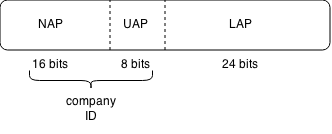
\includegraphics[width=200px]{images/bd_addr.png}
	\label{Bluetooth address}
	\caption{Bluetooth address definition}
  \end{center}
\end{figure}
\newpage
\subsubsection{Overview of Bluetooth security}

The basic security in Bluetooth is set up by the user, he has the choice between three different modes:
\begin{itemize}[nolistsep,noitemsep]
 	\item Silent: In this mode, the device will not initiate any connection. The only thing it does is monitoring the traffic.
 	\item Public: The device is discoverable by anyone around it having its bluetooth activated.
 	\item Private: The device will in that case only answer to device that it already paired with, thus making it (theoretically) only discoverable to known devices.\\
\end{itemize}

\noindent A Bluetooth device can implement four different security modes:

  \begin{itemize}[nolistsep,noitemsep]
  	\item Non Secure: As its name suggests there is no security.
  	\item Service-level enforced security mode: It establishes a non secure ACL (Asynchronous connectionless) link between the two devices willing to communicate. In order to introduce optional encryption, authentication and authorization, a request has to be made via L2CAP (Logical Link Control and Adaptation Protocol) connection-oriented or connection-less channel. This mode is used in versions 2.0 + EDR and below.
  	\item Link level enforced security mode: Once the ACL links are done then security procedures are initiated.
  	\item Service-level enforced security mode: This one is very similar to the second mode except that it introduces SSP (Secure Simple Pairing) and this is compatible only with Bluetooth versions from 2.1 + EDR.
  \end{itemize}

\subsubsection{Pairing process}
\label{subsubsec:pairingprocess}
SSP has been implemented in order to overcome the weakness of the 4 digits pass at the pairing time (only about 10.000 possibilities max) in addition to making the pairing process easier. \\
%Indeed, using an elaborated Bluetooth sniffer would allow to almost instantly find these digits and then bypassing the security.

Two devices pair by creating a shared key, called the Link key. This key will be used to authenticate and encrypt the data of two devices.
In order to do so, there are two possibilities: LMP-pairing (4-digits/pincode manner) or SSP. \\
Once this done, the two devices can store their mutual key in order to use it later for a re-pairing, making the connection much faster.\\
In LMP-pairing, the only thing that is not transmitted through the air is the 4 digits PIN code. The pairing process in this case works as follows: \\
The initiator will first generate a 16-bytes random number and then send it to the other device. Once received, both users will put in their PIN code which they will use to create an initialization key, the later will be converted into the actual LMP key. Finally, the two devices have to authenticate each other with their respective newly created LMP key. \\
A software created by Ellisys \cite{ellisys} allows an attacker that listens to the traffic to guess with the given information the 4 digits, thus making LMP useless. \\
An overview of the previously explained LMP pairing process is shown figure 2: 
\begin{figure}[!h]
  \begin{center}
	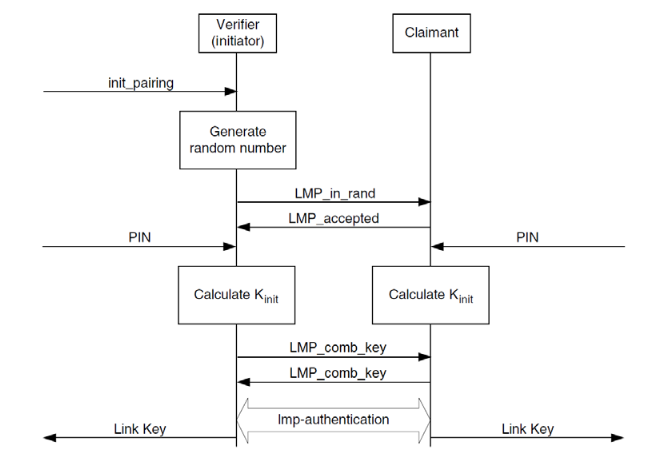
\includegraphics[width=350px]{images/haha.png}
	\label{LMP pairing}
	\caption{LMP pairing process}
	\caption*{\url{http://www.ellisys.com/technology/een_bt07.pdf}}
  \end{center}
\end{figure}

%Reference for SSP needed for the part underneath

SSP was then created, fixing the above vulnerability even though it is still possible to find this mechanism in many devices for backward compatibilities. \\
SSP is a new manner of generating a Link key by using Elliptic Curve. With this, it is possible to create a much bigger random number allowing a range of possible Link keys of $2^{128}$. This number is far too big to be brute forced. 

In order to create a public/private key pair (DHKey), SSP uses the famous Diffie-Hellmann algorithm with a 192-bits random number. The public key is transmitted over the air and can be seen by anyone, the private key is however kept secret for obvious security needs. 
Using two given key pairs A and B, there is a function that allows to result in a DHKey and only the two devices should be able to find it out. This function is F(Public A, Private B)=F(Public B, Private A). This very DHKey will be used in order to create the link key in between the two devices. \\ 
From there, the rest of the pairing process is similar to the LMP-pairing.

\newpage
\textbf{SAFER+ and protection against MiTM with SSP}\\

While BTLE uses AES, the older Bluetooth versions up to the 3.0+HS are using SAFER+ (Secure and Fast Encryption Routine) in order to provide authentication and key generation.\\
SAFER+ was candidate to the AES process and like it, it is a family of block ciphers using rounds and a block size of 128 bits.\\
In Bluetooth, SAFER+ is used for key derivation and authentication.\\
This algorithm uses a non-orthodox linear transformation to provide diffusion. It also use additive constant factors in order to avoid weak key generation.\\
Like in AES, it has two main components. The key-scheduling unit which is used in order to provide the round keys on the fly. The second one is called encryption data path, the latter will mix the plaintext with the "feedback" data from the previous rounds.\\

\noindent To be protected against MiTM attacks, SSP uses four association models:
\begin{enumerate}[nolistsep,noitemsep]
	\item The numeric comparison association model,  asks the user to compare numbers.
	\item Out Of Band (OOB) channel (NFC for example), used to check the integrity of a checksum.
	\item The Passkey Entry association model which is used when one of the device has input capabilities but no displays, in this case only the user with input capabilities will answer the 6-digit pass code.
	\item Finally, if one of the device has neither input nor output, and that OOB can't be used, then the JustWork association model is used, which is the weakest model as it simply asks the user to accept the connection.\\
\end{enumerate}
\noindent In SSP, there are 6 different phases in the pairing process:
\begin{enumerate}[nolistsep,noitemsep]
	\item Capabilities exchange: discovering devices or re-pairing ones will exchange their input/output capabilities.
	\item Public key exchange: Compute the private/public key using Diffie-Hellmann and give to each other their public keys. 
	\item Authentication stage 1: The protocol will depend on which of the four association model has been chosen. The aim of this stage is to be sure that nobody can eavesdrop the connection. 
	\item Authentication stage 2: There, the devices have exchanged their data and the integrity of each other is verified.
	\item Link key calculation: Using the previous steps, the Link key can be calculated (the DH key and nonces). It also needs the BD\_ADDR.
	\item Authentication and encryption: Now the encryption keys can be generated in order to encrypt all the data that will be exchanged between the two devices. \\
\end{enumerate}

\noindent The information provided in this section are based on K. Haataja et al. book chapter 2 \cite{btsecoverview} and wikipedia \cite{btwiki}.

\newpage
 %Florian
	\subsection{Ubertooth}
	\label{subsubsec:ubertooth}
Bluetooth technology is harder to sniff compared to other wireless protocols such as 802.11 that already have solutions for promiscuous packet sniffing. Because of how the way Bluetooth works it is harder to tap the communication between two devices. The devices need to pair before real message are being send. Normally you can only see the discovery messages with are used to find out which Bluetooth devices want to be found. Another problem is that Bluetooth devices can choose to stay hidden. \\
Due to frequency hopping it is hard to keep track of a device and listen to packet exchanged. However with the Ubertooth project it is now possible. To do so 3 parameters need to be known prior to be able to retrieve any information, the Lower Address Part (LAP), the Upper Address Part (UAP) and the clock CLKN that is the upper 26 bits of the CLK27 of the masters clock. The process to find this parameters is explained later on.
\\
Mike Ossman his project started in 2010 under the name of Ubertooth is dedicated to create and build a open source hardware that is able to follow and sniff Bluetooth communication. The Ubertooth was initially made to do just do following of Bluetooth devices. This can also be seen in the way the plug-ins for kismet work and the names of the tools made for the Ubertooth. The tools will be explained in section \ref{subsubsec:ubertooth_tools}. The latest release (Ubertooth 1) is capable of sniffing communication by identifying the right address and clock. The following sections explain how the clock and address are found and implications of finding these.

\subsubsection{Finding the UAP}
\label{subsubsec:finding_uap}
% This might also explain the clock searching process.
% But then I do not know why the clock still needs to found when you have the
% UAP
The UAP is the important to do anything interesting with Bluetooth. For instance it used to determine the hopping sequence that is used for the communication between two devices. It is 8 bits of the 48 bits $BD_ADDR$ (Bluetooth Device address). The LAP is transmitted in plain text. This makes it easy to find as it is present in all the packets. The First part is the NAP(Non-significant Adresss Part). This part is ignored because it is not needed for the initial communication. Because the UAP is only 8 bits it can be brute forced. This is not a good way to find it. Brute forcing is detectable and it will only work when the master is a connectible state. \pend
The Ubertooth is made to be a passive sniffer so this method is not used. One of the techniques used to determine the UAP is by using the HEC(Header Error Check). This is used to check if the header is received without errors. With this it is possible to determine what the are the unknown bits which will be the UAP. This header is send with each packet so it makes it easy to decode. The only problem is that it is XOR with a pseudo-random stream. To try and decode this is called "whitening". There are 64 possible streams it will use and this depends on which master clock is used. The lower 6 bits of are used to determine the. This clock is also used to make the hopping pattern. It will then generate 64 candidate UAP with each of the 64 streams. Sometimes the packets will have a CRC that can be used to check if the right stream is used to decode the packet. \pend
Another method is to perform a series of sanity checks on the packet format. The packet type can then be unwhiten. If the packet type is known some information can be derive such as the packet length. These information can confirm or deny a possible match. The problem with this is that false negatives can happen and it can eliminate UAP streams which are valid. This can happen, because the data that is decoded will be of wrong packet type and it will make the wrong conclusion on whether to or throw away this possible clock. This will lead to not finding any UAP for the master and the process will have to be restarted in order to find it. \pend %Harm
	\subsection{Sony Smartwatch SW2} %james
	\label{subsec:sw2}
The smartwatch that was chosen for this project is the Sony SmartWatch 2 \cite{sw2}. The SW2 uses Bluetooth 3.0, it is relatively cheap and programmable. The SDK (software development kit) has recently been updated and is easy to use. The SDK was used to make to make apps for the SW2. The installation guide can be found at this website \cite{sw2getstarted}. The SDK contains examples. These examples were used to generate traffic for the Ubertooth to sniff. The Ubertooth needs a decent amount of packets to decrypt the packets. Another benefit of using a self made application is that you exactly what is the content of the packets. This makes it easier to understand the traffic.
\begin{figure}[!h]
  \begin{center}
	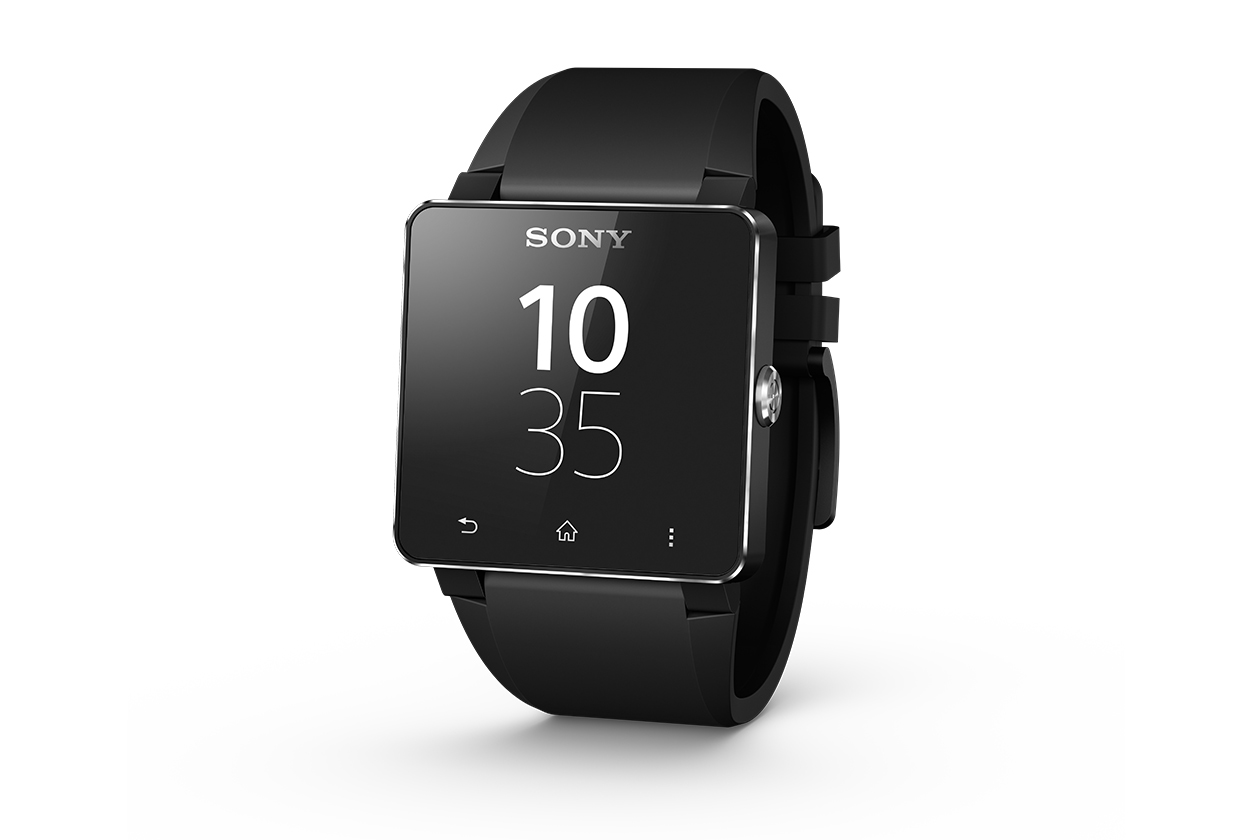
\includegraphics[width=200px]{images/sw2.jpg}
	\label{fig:sw2}
	\caption{Sony Smartwatch 2}
  \end{center}
\end{figure}
\newpage
All the Sony devices use an application called Smart Connect. This application keeps track of all the devices that want to make contact with the phone. It also keeps track of the applications that are installed on the watch. Whenever the pairing is stopped between the phone and the watch, all the previously installed applications are removed from the watch until these two devices are paired again.
\subsubsection{Smartwatch applications}
\label{subsubsec:sw_app}
%needs revision
The life cycle of a smartwatch app is about the same as an application on a phone or tablet. This can be seen in figure \ref{fig:sw2_lifecycle}. As stated before, the smartwatch apps only work when they are paired with the master device(the device which having the Smart Connect installed). When making an app, a few things are needed. First, register the app because it is needed for Smart Connect to find the app. \pend
Then update the AndroidManifest.xml file that defines the programmer main activity and some control features. After this, the app can be coded by including the mandatory classes to make the application compatible with SW2. \pend  
Sony has made a level of abstraction that makes it easy to send messages using intents. 
\begin{figure}
\begin{center}
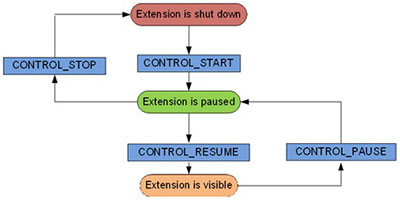
\includegraphics[scale=0.5]{images/applifecycle.jpg}
\end{center}
  \caption{Life cycle of a Sony smartwatch app}
  \label{fig:sw2_lifecycle}
  \captionsetup{font={footnotesize,bf,it}}
  \caption*{\url{https://developer.sony.com/develop/wearables/smartwatch-2-apis/guides/build-your-app/}}
\end{figure}
\newpage
\section{Methodology}		%us 3
This section describes the methodology followed to perform our analysis on Bluetooth communication. The first two parts will present how we investigated the different layers to analyse more efficiently the RF layer. The last one will present the methodology followed to investigate the pairing process between a phone and a smartwatch.


\subsection{The Ubertooth Tools}
\label{subsubsec:ubertooth_tools}
The Ubertooth comes with some tools to help you use the Ubertooth. This is done by the host code which is provided by project Ubertooth. 
The main tool we are using is \verb|ubertooth-rx|  this is the tool that we will be using the most. \verb|ubertooth-rx| is the tool that does all the hard stuff. It listens to all the packets send on the bandwidth and displays them. If you are using the default settings it will try to look for all the UAP of the devices. If you home in on a single device by using the option \verb|-l <LAP>| the tool will do a more in depth analysis. It will then use the given LAP and follow it. Then it will try to find UAP and the clock which will be explained in \ref{subsubsec:finding_uap}. When the program has found these two values it will have enough information to decrypt the packet. This packet will then be printed with. This is exactly where what we are looking for. \pend There is also a Kismet plug-in available which also uses \verb|ubertooth-rx|, but displays it in a better way in the Kismet interface. It also makes log files in pcap format which can then be used to analyse in Wireshark. The Kismet plug-in can only be used to discover all the Bluetooth devices in your neighbourhood and find their UAP. After it found the UAP it will not continue by trying to find the clock.

\begin{table}[!h]
\begin{tabular}{|l|l|}
\hline
Tool & Description \\
\hline
\verb|ubertooth-rx| & Passively scan for all the Bluetooth devices and try to find the UAP for them. \\
\hline
\verb|ubertooth-scan| & An active scan of all the Bluetooth devices in the neighbourhood.  \\
\hline
\verb|ubertooth-btle| & The Ubertooth low energy tool. \\
\hline
\end{tabular}
\caption{Ubertooth commands used during this project}
\label{tab:ubertooth_tools}
\end{table}
 
	%How was the experiment conducted comparison between hci layer and RF communication
	\subsection{The Bluetooth stack}
		
\subsubsection{RF layer}
	% How we Gather data form the ubertooth
	In order to eavesdrop a Bluetooth communication we used the Ubertooth 1 tool presented above. This tool is able to decode packet from a targeted Bluetooth communication.
	The LAP(Lower Address Part) was known for the two devices. As explained in the literature review the ubertooth tool retrieve the important parameters (UAP, clocks) used to sniff a connection thanks to that address. Once the tool was able to sniff and fallow a communication between the two devices it was possible for it to decode packets.
	In order to have relevant information the authors conducted experiments in a certain way. Indeed several captures have been performed recording:
\begin{itemize}
	\item[•] The pairing process between the two devices
	\item[•] The de-authentication process between two devices
	\item[•] The exchange of different data format (videos, pictures, notification) 
\end{itemize}
		 
\subsubsection{HCI layer}
	% How we Gather data form the hci
	Due to increasing use of Bluetooth; Android, since Android 4.4, have added a functionality available for developers to sniff Bluetooth packets at the HCI layer. This tool permits to monitor Bluetooth traffic in forms of pcaps logs for Wireshark. 
	The HCI layer is just above the LMP layer where authentication and encryption/encapsulation takes place. The data and messages exchanged at that layer are then in clear text and packets are not encapsulated. Then they are easily identifiable and easy to monitor.
	The experiments performed above at the RF layer have been performed in the same way (and at the same time) at the HCI layer. This as been done for analysis purposes.
			
		
	\subsection{Comparing data}	%find the relevance of the data found
		It is important to know if the data that the Ubertooth finds can also be seen in the HCI layer. This will confirm that the data that is shown by the Ubertooth is not bogus. Another reason to do this is that it was unknown what the the packets meant. The correlation between the two layers might give us more clarity about the things we were observing. \pend The data that was inspected were the packets that were not NULL or POLL. These packets have a payload and it is suspected to be received on the HCI level. To compare these packets, the Ubertooth and btsnoop\_hci.log from the android device have been used. Unfortunately, the packets on the HCI level have a higher level of abstraction and the packet types seen on the HCI layer are not the same as the packets that are sent over the RF layer. This means the correlation needs to be done with other means than looking at the packet types.\pend The correlation is done by looking at the timestamps. Both the HCI layer and the RF layer have timestamps in their messages. The assumption made is that the timestamps that is at which the packet arrives at the Ubertooth is not much different from the timestamp that is seen in HCI. By looking at the timestamps of the packets on the RF layer and assuming they will arrive at the HCI. The packets can then be linked to the packets seen on the HCI layer. \pend
This is the experiment that has been done to correlate the data from the Ubertooth with from the HCI:
\begin{itemize}
\item Install a slightly modified version of the example app called HelloActiveLowPowerActivity( the modification sends a message from the watch to android device once every second)
\item Start \verb|ubertooth-rx -l <LAP -u <UAP|. The UAP will also be given, because Ubertooth will not have to find the UAP by itself. 
\item Then start the smartwatch app that sends the messages
\item Both HCI layer and the Physical layer will be logged.
\end{itemize}
The interval between messages is chosen to be one second per message. With this many messages there is a higher chance of finding the the interesting packets. Sending it faster than this will make it harder to link the both layers together, because there will be too many packets with the same timestamp.
	
	\subsection{Investigating the pairing process}
		During the pairing process some critical information are exchanged. Indeed as explained in the literature review, master and slave are encrypting data thanks to several parameters common to each other: a key, a salt and a clock. These parameters are exchanged between master and slave during the pairing and this is what an attacker wants to know to be able to decrypt packets and understand what is exchanged.
Many papers have discussed the way to gather these information. Indeed, in order to retrieve them, an attacker would have first to see the pairing mechanism. That is why it is require to de-authenticate the user by making it believe his device is not working. Naturally the user will then re-pair himself with his device. This is where the attacker is able to see the different parameters exchanged. 
%This paper will explain how to retrieve these informations and explain how to use these information to decrypt a packet.
The pairing process is done in the Smart Connect application. This happens before any interaction with the smartwatch apps. This means that the apps have no control over the pairing process, but it is interesting to see what is sent over. 
To do so the pairing process have been looked from the HCI level of the device. At the HCI it is possible to see all the communication between the smartwatch and the device. During this process the LMP parameters are sent over line between the two devices. 
%From these parameters we can see that the encryption flag is turned on and that it uses SSP. (I think to put that in analysis in order to describe how the security is implemented)
\newpage
\section{Results and discussion}
result

		\subsection{Result Analysis}
		\subsection{Traffic investigation}
This section describes the traffic analysis done on the RF layer and the HCI layer. The third section describes how the data found at the two layer have been tried to be correlated.
\subsubsection{RF layer}
Regarding the RF layer a few messages can be seen. As shown in the appendix \ref{app:ubertooth} the most packets seen are the NULL and POLL messages, that are keep alive messages. During the captures the Ubertooth is only looking at channel 0 on which these packets are sent.

Some other packets are decoded by the Ubertooth and contains some data, the packets over the RF layer are of a different types. The packet decoded are of type DV/3-DH1, AUX1, AFH, DM1, HV1, DH5/3-DH5. An explanation of these packet types are explained in this appendix \ref{app:types} .

The only valuable information that could be output from this data analysis is that the packets sent between the smartwatch and the phone are fragmented as they contain different LLID parameters (which specifies if the payload is the start or the continuation of a L2CAP or LMP message). The packets are also encrypted.

\subsubsection{HCI layer}
From the HCI captures, some conclusions can be drawn. Indeed, during the pairing process, some parameters are negotiated regarding the future communication between the two devices. SSP introduces IO capabilities that permits to exchanged what would be the pairing model based on the capability of the master and slave device. 
\begin{figure}[!h]
  \begin{center}
	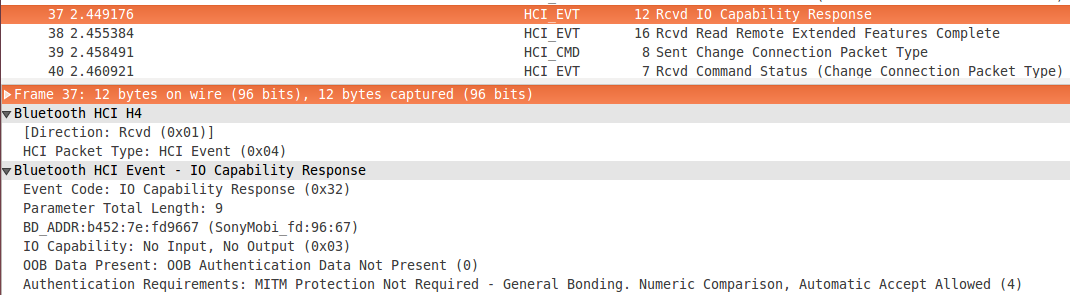
\includegraphics[width=270px]{images/IO_PARAM.png}
	\label{fig:io}
	\caption{IO capabilities found during the pairing process at the HCI layer}
  \end{center}
\end{figure}
The pairing process analysis shows that is based on JustWork mechanism. Indeed, as shown in \ref{fig:io} the Smartwatch claim not to have any input or output and that it does not have OOB authentication. Then the two devices agree to set up their connection with the JustWork mechanism that involves automatic accept of the numeric comparison. This mechanism is not protected from a MiTM attack \cite{MiTMjustworks}.

Then the LMP parameters \ref{fig:lmp} are exchanged to choose the LMP parameters that will be used during this communication. 
\begin{figure}[!h]
  \begin{center}
	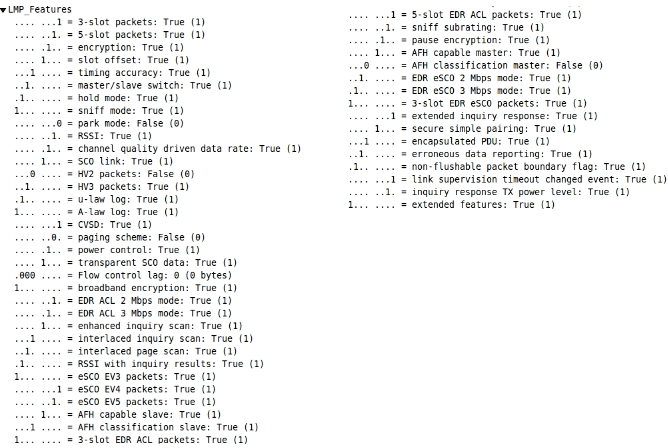
\includegraphics[width=270px]{images/LMP_PARAM.jpg}
	\label{fig:lmp}
	\caption{LMP Parameters found during the pairing process at the HCI layer}
  \end{center}
\end{figure}

From there, it is true to say that the communication uses SSP and is encrypted and encapsulated. It is even possible to retrieve the link keys used for encryption at this level. The link keys are always updated after a new pairing.

\subsubsection{Correlation of the two layers}

%Why cant we correlate the packet seen on Rf to hci? 
%Maybe we should trey to decrypt a packet using the key we found nat the hci. Just to proove that it is possible to decrypt the packets if we would have the key. ANd we would have the key maybe if the ubertooth was doing what we did.
<<<<<<< HEAD
Firstly the POLL and NULL packet are not available at the HCI layer because they are destined at the link controller layer so they cannot be used to correlated any information. 


\textbf{The 6 other types of packets found can or cannot be correlated?}

Another information that can be highlighted from the pairing process on the HCI, is that the master and the slave exchange information about what kind of packets are allowed during the communication. During this exchange the connection set up these packet types are disallowed. As you can see in appendix \ref{app:pairing}. The connection settings are set only to accept these kinds of packets shown. All the packets that are send over this channel which are not POLL or NULL are disallowed types. The reason why these packets are sent is unknown and their presence will be discussed in the next section.  \pend


\subsection{The rogue packets}
As already mentioned, there are some packets we cannot place. These packets can be found by the Ubertooth, but cannot be detected by the HCI. The issue with looking at the HCI level is that not all packets are seen at the HCI level. As it has been said in \ref{subsubsec:rflayer}. In fact, there may be some correlation, but it is not clear to guess that by just looking at them as a single set. A possible solution is to have a similar tool as the Ubertooth on the smartwatch to see what is sent at the same time. \\
As seen in appendix \ref{app:roguepackets}, there is an explanation of what information we get about the packet.
Looking at the first packet in appendix \ref{app:roguepackets} there are a few things that can be seen. The data is always doubled and the packet is divided in a few fields. Type, LT\_ADDR, flow, payload length and data. The first line contains some information about the packet. The most important values from this information are:
=======
Firstly the POLL and NULL packet are not available at the HCI layer. They are destined and processed at the link controller layer so they cannot be seen. With this said these package will have no effect on the correlation between what is seen on the Ubertooth and in the HCI. More interesting are the other packages mentioned in 

\subsection{The rogue packets}
As already mentioned, there are some packets we cannot place. These are packets that can be found by the Ubertooth, but cannot be detected by the HCI. These messages are handled in the LC see figure \ref{subsubsec:rflayer}.
Some examples are seen in appendix \ref{app:roguepackets}.
Looking at the first packet in appendix \ref{app:roguepackets} there are a few things that can be seen. The packets with data are always doubled. The reason for this is unknown. The unwhitened packet is divided in a few fields. Type, LT\_ADDR, flow, payload length and data. The first line contains some information about the packet. The most important values from this information are:
>>>>>>> a006064e2425f766d9ded6d518c945710e757ac5
\begin{itemize} 
\item The \textbf{ch}, this is the channel in which the packet was found.
\item The \textbf{LAP}, which is the sender's lower address part.
\end{itemize}
The reason that the type has two values is that for different data rates the packet type can differ. The SW2 has no voice capabilities and knows high data transfer rate. In specifications table that can be found 308 in the last column. So the packet types will always be the latter of the two types given.
The LT\_ADDR is used to determine which is used by each receiving device to determine if the packet addressed to them, but it is also used ffor internal routing.
The LLID is the (Logical Link Identifier)
To analyse the payload the authors have tried to decode these packets using the key exchanged during the pairing process but have failed.

		\subsection{Problems encountered}
		\label{subsec:problems}
There are a few problems we have encountered during the project. The main problem is that we cannot see the most important data that is send. This being the pairing process and the data that is exchanged between the smartwatch and an other android device. The only traffic visible are the poll and null messages that are send over channel 0. This is because the Ubertooth cannot follow the faster data rates that are being exchanged. Another problem  is identifying. 
		\subsection{Discussion}
		discussion

\newpage
\section{Conclusion and Future work}
The Ubertooth is not useful for inspecting the communication between the SW2 and another device. Packets that can be seen with the Ubertooth are the discovery, keep alive and  "rogue" packets. This makes the Ubertooth not very useful to do any kind of analysis about the traffic between the SW2 and another device. This is because the SW2 uses Bluetooth 3.0. With Bluetooth 3.0  most of the packets are send with a data rate that Ubertooth cannot follow. On the other hand we can confirm that the Ubertooth can be used follow discoverable Bluetooth devices on the network and can uniquely identify them. \pend 
However some interesting point came up when investigating the HCI layer. First of all the SW is using the JustWork protocol. Which means that no PIN code exchanged/comparison is needed between the two devices. That makes the pairing process weak against MiTM attack. In order to solve this issue Sony should force the use of a stronger SSP association model such as NFC (already available) or the Passkey entry.   

Ubertooth is still under development. The tools are still being improved and there is not enough documentation about how to properly use them. With time this will get better and seeing what it can already do with Bluetooth 4.0 it is nice tool for a variety for experiments. But for Bluetooth 3.0 it is not a very useful tool. However a solution could be to use a tool such as the FTS4BT Frontline sniffer \cite{FTS4BT} that are able to sniff any Bluetooth protocols. The only issue with this hardware is that it is really expensive. Then it was not possible to acquire this kind of hardware for this project due to budget issue.
\pend
In the future experiments can be done with a smartwatch that Bluetooth 4.0 Low energy which transfer data in low energy mode. The Ubertooth has good tools to work with this and it is still nice to look what you can do with it.
Further inspecting what the Ubertooth can and cannot detect. One idea for this is to manually setting up a connection between devices and send different kinds of data. During the project all connections have been setup automatically. \pend
The Smart Connect app can be inspected as well. This app controls all the smartwatch apps and plays a pivotal role in how the smartwatch works. Inspecting this might surface more vulnerabilities not only in the smartwatch, but also other Bluetooth devices. \pend
Lastly the MITM attack can be performed. It has already been shown that if your device uses JustWork for pairing that it is vulnerable. It will be interesting to see how the smartwatch apps will react to a MITM. To make this possible a normal dongle should be bought and a Bluetooth spoofing program.

\newpage

\vspace*{2\baselineskip} % Whitespace between location/year and editors


\bibliography{bib}{}
\bibliographystyle{plain}


\end{document}